\chapter{확률 질량 함수}
\index{확률 질량 함수 (probability mass function)}

이번 장에서 사용되는 코드는 {\tt probability.py}에 있다.
코드를 다운로드하고 작업하는 것에 대한 정보는 ~\ref{code}을 참조한다.

\section{Pmf}
\index{Pmf}

분포를 표현하는 또다른 방식은 {\bf 확률 질량 함수(probability mass function)} (PMF)로 각 값을 확률로 매핑한다. 
{\bf 확률(probability)}은 표본 크기 {\tt n}의 일부로서 표현되는 빈도다. 
빈도에서 확률을 얻기 위해서, {\tt n}으로 나누는데 이를 {\bf 정규화(normalization)}라고 부른다.

\index{빈도 (frequency)}
\index{확률 (probability)}
\index{정규화 (normalization)}
\index{PMF}
\index{확률 질량 함수 (probability mass function)}

Hist가 주어지면, 각 값에 확률값을 매핑하는 딕셔너리를 만들 수 있다.
\index{Hist}

%
\begin{verbatim}
n = hist.Total()
d = {}
for x, freq in hist.Items():
    d[x] = freq / n
\end{verbatim}
%

혹은 {\tt thinkstats2}에서 제공하는 Pmf 클래스를 사용할 수도 있다.
Hist와 마찬가지로, Pmf 생성자는 판다스, 시리즈, 딕셔너리, Hist, 다른 Pmf 객체를 받을 수 있다.
다음에 간단한 리스트를 입력값으로 받는 예제가 있다.

%
\begin{verbatim}
>>> import thinkstats2
>>> pmf = thinkstats2.Pmf([1, 2, 2, 3, 5])
>>> pmf
Pmf({1: 0.2, 2: 0.4, 3: 0.2, 5: 0.2})
\end{verbatim}

Pmf는 정규화 과정을 거쳐 전체 확률값이 1이 된다.

Pmf와 Hist 객체는 많은 점에서 비슷하다; 사실, 공통 부모 클래스에서 많은 메쏘드를 상속받았다.
예를 들어, {\tt Values}와 {\tt Items} 메쏘드는 두 객체 모두에 동일한 방식으로 동작한다.
가장 큰 차이점은 Hist가 값을 정수형 계수기(integer counter)로 매핑한다는 것이고; 
Pmf는 값을 부동소수점 확률값으로 매핑한다는 것이다. 
\index{Hist}

값과 연관된 확률값을 조회하려면, {\tt Prob}를 사용한다.:
%
\begin{verbatim}
>>> pmf.Prob(2)
0.4
\end{verbatim}

꺾쇠 연산자도 동등한 기능을 한다.
\index{꺾쇠 연산자 (bracket operator)}

\begin{verbatim}
>>> pmf[2]
0.4
\end{verbatim}

기존 Pmf를 값과 연관되어 있는 확률값을 증가시킴으로써 변경할 수 있다.
%
\begin{verbatim}
>>> pmf.Incr(2, 0.2)
>>> pmf.Prob(2)
0.6
\end{verbatim}

혹은 확률에 일정량을 곱할 수도 있다.
%
\begin{verbatim}
>>> pmf.Mult(2, 0.5)
>>> pmf.Prob(2)
0.3
\end{verbatim}

만약 Pmf를 변경하면, 결과는 정규화되지 않을지도 모른다; 즉, 확률값을 다 합하면 1이 되지 않을지도 모른다.
확률값을 합한 결과를 반환하는데 사용되는 {\tt Total} 메쏘드를 호출해서 확인한다. 

%
\begin{verbatim}
>>> pmf.Total()
0.9
\end{verbatim}

다시 정규화하기 위해서, {\tt Normalize}를 호출한다:
%
\begin{verbatim}
>>> pmf.Normalize()
>>> pmf.Total()
1.0
\end{verbatim}

Pmf 객체는 {\tt Copy} 메쏘드를 제공하는데, 이를 통해서 원본에 영향을 주지않고, 사본을 만들고 변경 작업을 할 수 있다.
\index{Pmf}

이번 절에 표기법이 일관성을 갖지 않는 것처럼 보일지도 모르지만 체계가 있다;
Pmf를 클래스 명칭으로, pmf는 클래스의 인스턴스로, PMF는 확률질량함수에 대한 수학적 개념으로 각각을 표기하는데 사용한다.

\section{PMF 플롯으로 그리기}
\index{PMF}

{\tt thinkplot}은 Pmf 플롯을 그리는 두가지 방식을 제공한다.
\index{thinkplot}

\begin{itemize}

\item Pmf를 막대그래프로 그리기 위해서 {\tt thinkplot.Hist}을 사용한다.
만약 Pmf에 값의 개수가 작다면 막대그래프가 가장 유용한다.
\index{막대그래프 (bar plot)}
\index{그래프 (plot)!막대 (bar)}

\item 계단 함수로 Pmf를 그래프 그리기 위해서는, {\tt thinkplot.Pmf}을 사용할 수 있다.
만약 값이 많고, Pmf가 매끄럽다면(smooth) 탁월한 선택이 된다. 이 함수는 Hist 객체에서도 동작한다.
\index{선그래프 (line plot)}
\index{그래프 (plot)!선 (line)}
\index{Hist}
\index{Pmf}

\end{itemize}

추가로, {\tt pyplot}은 {\tt hist} 함수를 제공하는데 값(value) 시퀀스를 받아서
히스토그램을 계산하고, 그래프로 그린다.
Hist 객체를 사용하기 때문에, {\tt pyplot.hist}은 사용하지 않는다.
\index{pyplot}

\begin{figure}
% probability.py
\centerline{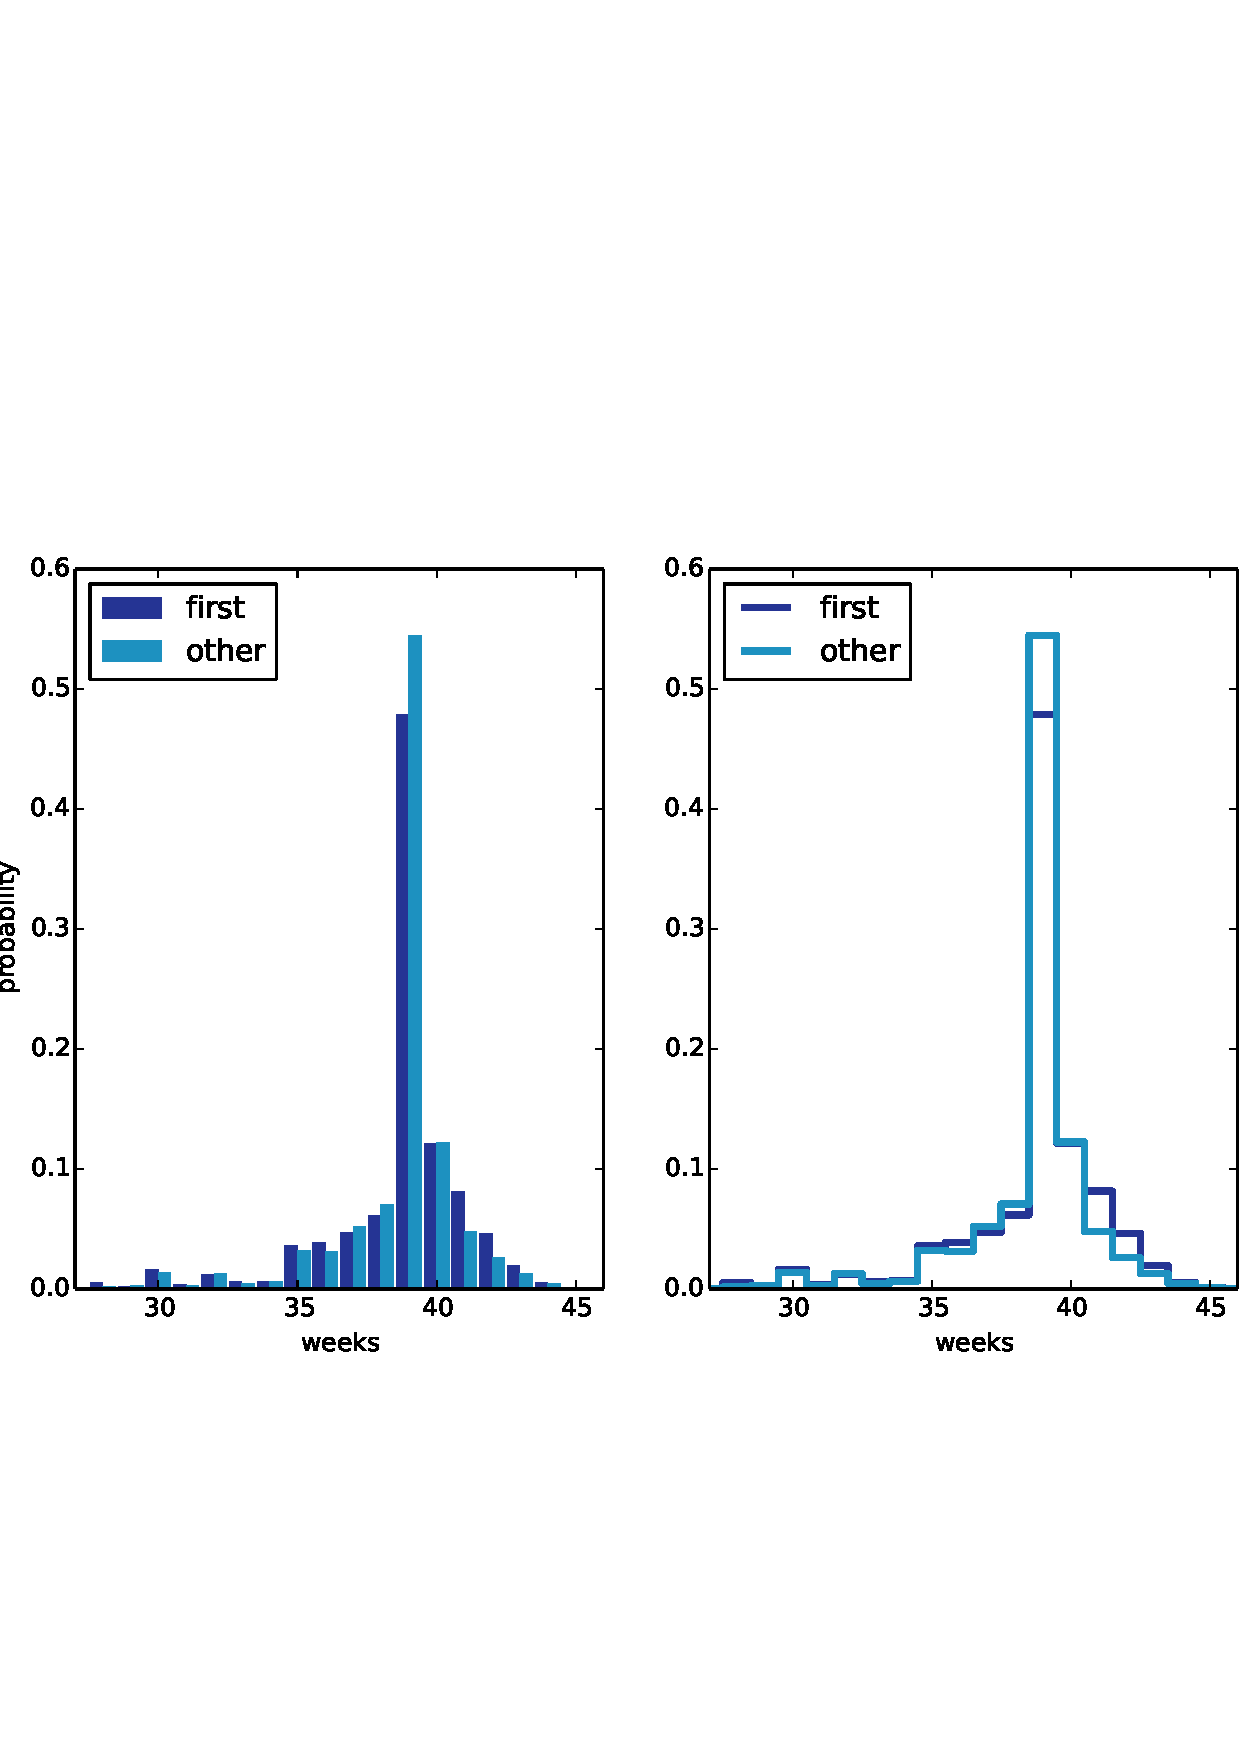
\includegraphics[height=3.0in]{figs/probability_nsfg_pmf.pdf}}
\caption{막대 그래프와 계단 함수를 사용하여, 첫째 아기와 첫째가 아닌 아기에 대한 임신기간 PMF.}
\label{probability_nsfg_pmf}
\end{figure}
\index{임신기간 (pregnancy length)}
\index{기간 (length)!임신 (pregnancy)}

그림~\ref{probability_nsfg_pmf}은 막대그래프(왼쪽)와 계단함수(오른쪽)를 사용해서 첫째 아이와 첫째가 아닌 아이에 대한
임신기간 PMF를 보여준다.
\index{임신기간 (pregnancy length)}

히스토그램 대신에 PMF 플롯을 그려서, 표본차이로 오도되지 않고 두 분포를 비교할 수 있다.
그림을 해석하면, 첫번째 아이는 다른 아이들보다 정시(39주차)에 출산하지 않고, 늦게(41, 42주차) 출산할 것 같다.

그림~\ref{probability_nsfg_pmf}을 생성하는 코드가 다음에 있다:

\begin{verbatim}
    thinkplot.PrePlot(2, cols=2)
    thinkplot.Hist(first_pmf, align='right', width=width)
    thinkplot.Hist(other_pmf, align='left', width=width)
    thinkplot.Config(xlabel='weeks',
                     ylabel='probability',
                     axis=[27, 46, 0, 0.6])

    thinkplot.PrePlot(2)
    thinkplot.SubPlot(2)
    thinkplot.Pmfs([first_pmf, other_pmf])
    thinkplot.Show(xlabel='weeks',
                   axis=[27, 46, 0, 0.6])
\end{verbatim}

{\tt PrePlot} 메쏘드는 옵션 매개변수 {\tt rows}와 {\tt cols}을 받아서 
그림 격자(grid)를 만드는데 이경우 한 행에 그림 두개를 넣는 격자가 된다.
첫번째 그림(왼쪽)은 {\tt thinkplot.Hist}을 사용해서 앞에서 봤던 Pmf를 화면에 출력한다. 

\index{thinkplot}
\index{Hist}

{\tt PrePlot}에 두번째 호출로 색깔 생성자를 초기화한다. 그리고 나서 
{\tt SubPlot}이 두번째 그림(오른쪽)으로 바꿔서, {\tt thinkplot.Pmfs}을 사용해서 Pmf를 화면에 출력한다.
{\tt axis}을 사용해서 그림 두개 모두 동일한 축(axis)에 놓여지도록 확실히 한다.
그림 두개를 비교하려고 한다면, 축을 통일하는 것이 좋다.


\section{다른 시각화 방법}
\label{visualization}

히스토그램과 PMF은 데이터를 탐색하고 패턴과 관계를 식별하는데 유용하게 사용된다. 데이터에서 무슨 정보가 담겨져있고, 어떻게 돌아가는지 아이디어를 얻게 된다면, 다음 단계는 최대한 깔끔하게 식별한 패턴화할 수 있는 시각화 설계하는 것이다. 

\index{탐색적 자료 분석 (exploratory data analysis)}
\index{시각화 (visualization)}

NSFG데이터에서 분포에서 가장 큰 차이는 모드(최빈치)에 있다. 그래서, 그래프에서 이 부분만을 확대하여 들여다보고, 차이를 강조하도록 자료를 변환하는 것이 의미가 있다.

\index{가족 성장 국가 조사 (National Survey of Family Growth)}
\index{NSFG}

\begin{verbatim}
    weeks = range(35, 46)
    diffs = []
    for week in weeks:
        p1 = first_pmf.Prob(week)
        p2 = other_pmf.Prob(week)
        diff = 100 * (p1 - p2)
        diffs.append(diff)

    thinkplot.Bar(weeks, diffs)
\end{verbatim}

상기 코드에서 {\tt weeks}가 임신주 범위다; {\tt diffs}는 퍼센트에서 두 PMF간 차이가 된다.  
그림~\ref{probability_nsfg_diffs}는 막대그래프로 결과를 보여준다.
그림이 패턴을 좀더 명확하게 한다: 첫째 아이는 임신 39주차에 덜 태어날 것 같고, 임신 41, 42주차에 더 태어날 것 같다.
\index{thinkplot}

\begin{figure}
% probability.py
\centerline{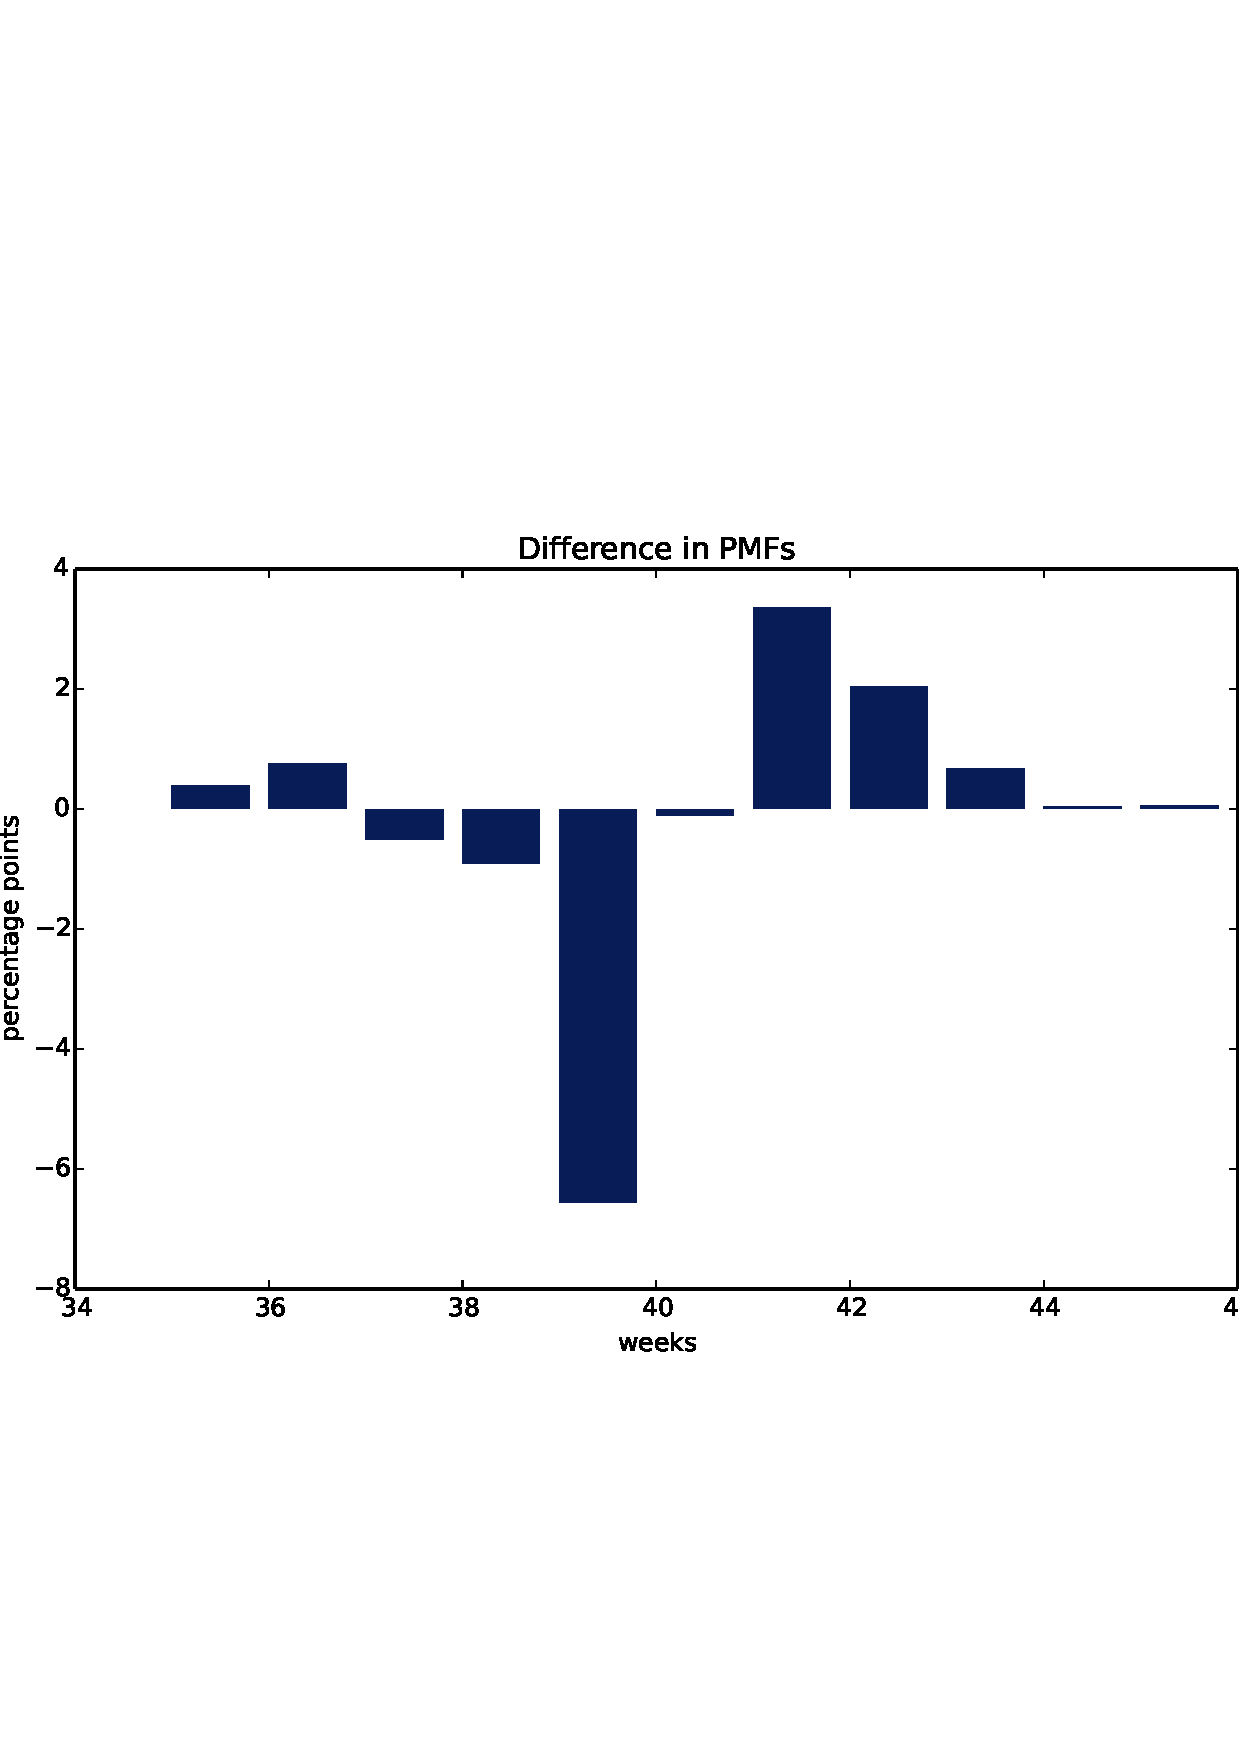
\includegraphics[height=2.5in]{figs/probability_nsfg_diffs.pdf}}
\caption{주별 백분율점(percentage point)으로 나타낸 차이.}
\label{probability_nsfg_diffs}
\end{figure}

지금까지 결론을 잠정적으로 내렸다. 동일한 데이터셋을 사용해서 명백하게 차이를 식별하고 나서 차이를 명확하게 만드는 시각화 방식을 선택했다. 효과 차이가 실질적인지 확실하다고 할 수는 없다; 확률변동(random variation)일 수도 있다. 나중에 이 문제를 다시 다룰 것이다.


\section{학급 크기 패러독스 (class size paradox)}
\index{학급 크기 (class size)}

진도를 더 나가기 전에, Pmf 객체를 가지고 할 수 있는 한가지 계산(computation)을 시연하고자 한다; 다음 예제를 ``학급 크기 패러독스(class size paradox)''라고 명명한다.
\index{Pmf}

많은 미국 대학에서, 학생대교수 비율은 약 10:1이 된다. 
하지만 종종 학생들이 평균 학급크기가 10보다 큰 것을 발견하고 놀라곤 한다.
불일치에 대한 두가지 이유가 있다.

\begin{itemize}

\item 학생들이 학기당 일반적으로 4--5 과목을 수강하지만, 교수는 1 혹은 2 교과목만 가르친다. 

\item 적은 학급 수업을 즐기는 학생 숫자는 적지만, 큰 학급 수업에 학생수는 많다.
\end{itemize}

첫 이유는 명확하지만, 두번째 이유는 다소 모호하다. 사례를 살펴보자. 대학에서 다음과 같은 학급 크기 분포로 한 학기에 65 교과목을 개설한다고 가정하자.

%
\begin{verbatim}
 size      count
 5- 9          8
10-14          8
15-19         14
20-24          4
25-29          6
30-34         12
35-39          8
40-44          3
45-49          2
\end{verbatim}

만약 학교 총장에게 평균 학급크기를 물어본다면, 총장은 PMF를 생성하고, 평균을 계산하고 나서 학급 평균 크기가 23.7이라고 보고한다. 다음에 코드가 있다.

\begin{verbatim}
    d = { 7: 8, 12: 8, 17: 14, 22: 4, 
          27: 6, 32: 12, 37: 8, 42: 3, 47: 2 }

    pmf = thinkstats2.Pmf(d, label='actual')
    print('mean', pmf.Mean())
\end{verbatim}

하지만, 학생집단을 대상으로 수업에 학생이 있는지 물어보고, 평균을 계산한다면, 평균 학급크기가 더 크다고 생각할 것이다. 얼마나 더 큰지 살펴보자.

먼저, 학생들이 관측한 분포를 계산하자. 여기서 각 학급 크기와 연관된 확률은 학급에 있는 학생으로 ``편의(bias)''가 있다.

\index{관측자 편의 (observer bias)}
\index{편의 (bias)!관측자 (observer)}

\begin{verbatim}
def BiasPmf(pmf, label):
    new_pmf = pmf.Copy(label=label)

    for x, p in pmf.Items():
        new_pmf.Mult(x, x)
        
    new_pmf.Normalize()
    return new_pmf
\end{verbatim}

각 학급 크기 {\tt x}마다, 확률값에 학급 크기를 관측한 학생수 {\tt x}를 곱한다. 결과는 편의분포를 나타내는 새로운 Pmf가 된다.

이제 실제와 관측된 분포 모두를 플롯 그래프로 그릴 수 있다.
\index{thinkplot}

\begin{verbatim}
    biased_pmf = BiasPmf(pmf, label='observed')
    thinkplot.PrePlot(2)
    thinkplot.Pmfs([pmf, biased_pmf])
    thinkplot.Show(xlabel='class size', ylabel='PMF')
\end{verbatim}

\begin{figure}
% probability.py
\centerline{\includegraphics[height=3.0in]{figs/class_size1.pdf}}
\caption{실제값과 학생이 관측한 값에 대한 학급크기 분포.}
\label{class_size1}
\end{figure}

그림~\ref{class_size1}은 결과를 보여준다. 편의된 분포에서 작은 학급은 더 작고, 큰 학급은 더 많다. 편의된 분포 평균은 29.1로 실제 평균값보다 약 25\%더 많다. 

이 연산을 거꾸로 하는 것도 또한 가능하다. 대학 학급 크기 분포를 알고자 한다고 가정하자. 하지만, 대학 총장으로부터 신뢰성 있는 자료를 얻을 수는 없다. 대안은 무작위 학생 표본을 골라 학급에 학생수가 얼마인지 설문하는 것이다.
\index{편의 (bias)! 오버샘플링 (oversampling)} 
\index{오버샘플링 (oversampling)}

결과는 앞선 살펴봤던 이유로 편의가 있을지 모르지만, 이것을 사용해서 실제 분포를 추정한다. 다음에 Pmf 불편의(unbiased) 함수가 있다. 

\begin{verbatim}
def UnbiasPmf(pmf, label):
    new_pmf = pmf.Copy(label=label)

    for x, p in pmf.Items():
        new_pmf.Mult(x, 1.0/x)
        
    new_pmf.Normalize()
    return new_pmf
\end{verbatim}

{\tt BiasPmf} 함수와 비슷하다; 유일한 차이점은 곱하는 대신에 각 확률값을 {\tt x}로 나눈다는 것이다.

\section{데이터프레임 인덱싱 (DataFrame indexing)}

\ref{dataframe} 절에서 판다스 데이터프레임을 읽고, 데이터프레임을 사용해서 데이터 열(칼럼)을 선택하고 변경했다. 
이제 행선택을 살펴보자.
NumPy 난수 행렬을 생성하고, 이것을 사용해서 데이터프레임으로 초기화한다.

\index{넘파이 (NumPy)}
\index{판다스 (pandas)}
\index{데이터프레임 (DataFrame)}

\begin{verbatim}
>>> import numpy as np
>>> import pandas
>>> array = np.random.randn(4, 2)
>>> df = pandas.DataFrame(array)
>>> df
          0         1
0 -0.143510  0.616050
1 -1.489647  0.300774
2 -0.074350  0.039621
3 -1.369968  0.545897
\end{verbatim}

초기 설정값(by default)으로 행과 열 모두 0에서 시작하는 숫자로 번호가 매겨진다. 하지만, 열이름을 지정할 수 있다.

\begin{verbatim}
>>> columns = ['A', 'B']
>>> df = pandas.DataFrame(array, columns=columns)
>>> df
          A         B
0 -0.143510  0.616050
1 -1.489647  0.300774
2 -0.074350  0.039621
3 -1.369968  0.545897
\end{verbatim}

행이름도 지정할 수 있다. 행이름 집합을 {\bf index}라고 한다; 
행이름 자체는 {\bf labels}이라고 한다.

\begin{verbatim}
>>> index = ['a', 'b', 'c', 'd']
>>> df = pandas.DataFrame(array, columns=columns, index=index)
>>> df
          A         B
a -0.143510  0.616050
b -1.489647  0.300774
c -0.074350  0.039621
d -1.369968  0.545897
\end{verbatim}

앞장에서 살펴보았듯이, 단순 인덱싱으로 열을 선택하면 시리즈를 반환한다.

\index{시리즈 (Series)}

\begin{verbatim}
>>> df['A']
a   -0.143510
b   -1.489647
c   -0.074350
d   -1.369968
Name: A, dtype: float64
\end{verbatim}

레이블(label)로 행을 선택하려면 {\tt loc} 속성을 사용하면 되고 시리즈를 반환한다.  

\begin{verbatim}
>>> df.loc['a']
A   -0.14351
B    0.61605
Name: a, dtype: float64
\end{verbatim}

레이블(label) 보다 행의 정수 위치정보를 알고 있다면, {\tt iloc}속성을 사용하고, 실행 결과로 시리즈를 반환한다.

\begin{verbatim}
>>> df.iloc[0]
A   -0.14351
B    0.61605
Name: a, dtype: float64
\end{verbatim}

또한 {\tt loc}는 레이블 리스트를 인자로 받고, 결과로 데이터프레임을 반환한다.

\begin{verbatim}
>>> indices = ['a', 'c']
>>> df.loc[indices]
         A         B
a -0.14351  0.616050
c -0.07435  0.039621
\end{verbatim}

마지막으로 레이블(label)로 행 범위를 선택하는데 슬라이스를 사용할 수 있다.

\begin{verbatim}
>>> df['a':'c']
          A         B
a -0.143510  0.616050
b -1.489647  0.300774
c -0.074350  0.039621
\end{verbatim}

혹은 정수 위치정보를 사용할 수도 있다.

\begin{verbatim}
>>> df[0:2]
          A         B
a -0.143510  0.616050
b -1.489647  0.300774
\end{verbatim}

어느 경우든지 관계없이 결과는 데이터프레임이 된다. 하지만 첫번째 결과는 슬라이스 끝값을 포함하지만, 두번째는 끝값을 포함하지 않는 것을 주목하라.
\index{데이터프레임 (DataFrame)}

저자 충고: 만약 행에 단순히 정수값이 아닌 레이블(label)이 있다면, 레이블을 일관되게 사용하고 정수 위치정보 사용을 피하라.


\section{연습 문제}
이번 연습문제 대한 해답은 \verb"chap03soln.ipynb" 파일과 
\verb"chap03soln.py" 파일에 담겨있다.

\begin{exercise}
만약 자녀에 대해서, 얼마나 많은 자녀가 있는지 묻는다면, 학급 크기 패러독스 같은 것이 나타난다. 많은 자녀를 갖는 가족이 표본에 더 잘 나타날 것 같고 자녀가 없는 가족이
표본에 나타날 가능성은 없다.

\index{관측자 편향}
\index{편향!관측자}

NSFG 응답자 \verb"NUMKDHH" 변수를 사용해서 
가구에서 18세 이하 자녀수에 대한 실제 분포를 생성하라.

이제 만약 자녀에 대해서, 18세 이하 (본인 포함) 얼마나 많은 자녀가 있는지 묻는다면,
보게될 편향된 분포를 계산하라.

실제 분포와 편향된 분포를 도식화하고 평균을 계산하라. 
출발장소로 \verb"chap03ex.ipynb" 파일을 사용할 수 있다.
\end{exercise}


\begin{exercise}
\index{평균 (mean)}
\index{분산 (variance)}
\index{PMF}

\ref{mean}~절에서 구성요소를 더해가고 $n$으로 나눠서 표본 평균을 계산했다.
만약 PMF가 주어지면, 여전히 평균을 계산할 수 있으나, 과정은 다소 차이가 난다:
%
\[ \xbar = \sum_i p_i~x_i \]
%
여기서, $x_i$는 PMF에 있는 유일한 값이고, $p_i=PMF(x_i)$.
마찬가지로, 다음과 같이 분산을 계산할 수 있다:
%
\[ S^2 = \sum_i p_i~(x_i - \xbar)^2\]
% 
Pmf 객체를 인자로 받아 평균과 분산을 계산하는 함수를 
{\tt PmfMean} 와 {\tt PmfVar} 으로 이름지어 작성하시오.
작성한 메쏘드를 테스트하기 위해서, Pmf에서 제공하는 
{\tt Mean}, {\tt Var} 메쏘드와 일치하는지 검사하라.
\index{Pmf}

\end{exercise}


\begin{exercise}
저자는 ``첫째 아이가 좀더 늦게 태어날 것 같은가?'' 라는 질문으로 시작했다.
이 질문을 다루는데, 아이 집단간에 평균에 차이를 계산했다.
하지만, {\em 동일 여성에 대해} 첫째 아이와 다른 아이 사이에 차이가 있을 수 있다는 가능성을 간과했다.

이 질문을 다루는데, 적어도 아이가 두명인 응답자를 선택하고 
쌍별 차이(pairwise difference)를 계산한다.
이 질문 구성이 다른 결과를 도출해 내는가?

힌트: {\tt nsfg.MakePregMap}을 사용한다.
\end{exercise}


\begin{exercise}
\label{relay}

대부분의 도보경주(foot race)에서 모든 사람이 같은 시간에 출발한다.
만약 빠른 주자라면, 초반 경주에서 많은 사람을 앞질러 간다.
하지만, 몇 마일 지난 후에 주위 모든 사람은 같은 속도록 달려간다.

\index{계주}

저자가 처음으로 장거리 (209마일) 계주를 뛰었을 때, 저자는 특이한 현상을 알아챘다:
저자가 다른 주자를 따라 잡았을 때, 저자는 통상 훨씬 더 빠르고,
또다른 주자가 저자를 따라 잡았을 때, 또다른 주자가 저자보다 훨씬 더 빠르다.

처음에, 저자는 선수속도 분포가 이봉이라고 생각했다;
즉, 속도가 느린 주자와 속도가 빠른 주자, 하지만 저자와 같은 속도는 소수.

그리고 나서, 저자가 학급크기 효과와 유사한 편향의 희생자임을 인식하게 되었따.
경주는 두가지 방식으로 일반적이 않다: 스태거드 스타트(Staggered Start)를 사용해서, 다른 시점에 팀을 지어 출발한다; 그래서 다른 수준의 능력을 갖는 주자가 많은 팀에 포함된다.

\index{편향!선택} \index{선택 편향}

결과적으로, 주자는 속도와 장소에 거의 관계없이 경주과정을 통해서 쭉 펼쳐지게 된다.
저자가 경주에 참가했을 때, 저자 주위 참가자는 (상당히) 경주에 참가한 임의 표본이다.

그래서, 편향은 어디서 나오는 것일까? 경주를 진행하는 동안, 저자가 경주자를 추월하고, 추월당하는 가능성은 속도 차이에 비례한다. 저자가 느린 주자를 따라잡을 것 같고, 
빠른 주자에 따라잡힐 듯 하다. 하지만, 같은 속도를 갖는 주자는 서로를 보지 못할 듯 하다.

{\tt ObservedPmf}로 불리는 함수를 작성한다.
작성한 함수는 주자 속도와 달리는 관측자의 속도에 대한 실제 분포를 나타내는 Pmf를 인자로 받고, 관측자가 본 경주자의 분포를 나타내는 새로운 Pmf를 반환한다.

\index{관측자 편향}
\index{편향!관측자}

작성한 함수를 테스트하는데, {\tt relay.py}를 사용할 수 있는데,
마이애미 Dedham에서 열린 10 킬로미터 제임스 조이스 경주(James Joyce Ramble)에서 
나온 결과를 읽고 각 주자의 속도를 mph로 변환한다.

만약 7.5 mph로 해당 집단 주자와 계주를 달린다면, 관측할 속도 분포를 계산하시오.
이 연습문제 대한 해답은 \verb"relay_soln.py"에 나와있다.
\end{exercise}


\section{용어사전}

\begin{itemize}

\item 확률질량함수 (Probability mass function, PMF): 값을 확률로 매핑하는 함수로 분포를 표현.
\index{PMF}
\index{확률질량함수 (probability mass function)}

\item 확률 (probability): 
표본크기의 일부로 표현되는 빈도수.
\index{빈도 (frequency)}
\index{확률 (probability)}

\item 정규화 (normalization): 
확률값을 얻기 위해서 표본 크기로 빈도수를 나누는 과정.
\index{정규화 (normalization)}

\item 인덱스 (index): 
판다스 데이터프레임에서, 인덱스는 행 레이블(label)을 포함하는 특별한 열(칼럼)이다.
\index{판다스 (pandas)}
\index{데이터프레임 (DataFrame)}

\end{itemize}
